% ---------------------------------------------------------------------------
% Varaksin contribution packet, for integration into the Shiianov/Sverdlov paper.
%
% PURE ASCII BY DESIGN. gena_paper.tex is UTF-8; the Zapiski template requires
% CP1251. Anything non-ASCII corrupts in one of the two. Paste as-is.
%
% Numbering continues the existing scheme (E1-E5 -> E6-E9) so the experiments
% read as one programme. Same model, same revision bb6621b6..., same
% core_block[-1] hook, same inference-only protocol.
%
% PART 1 is drop-in text.  PART 2 is notes for the lead author -- DO NOT PASTE
% PART 2; it lists the edits the merge requires on the E1-E5 side, and why.
% ---------------------------------------------------------------------------
\documentclass[11pt,a4paper]{article}
\usepackage[margin=2.4cm]{geometry}
\usepackage{booktabs,multirow,graphicx,amsmath,amssymb}
\usepackage[colorlinks=true,linkcolor=black,urlcolor=blue]{hyperref}
\setlength{\parskip}{2pt}
\title{\vspace{-1.6cm}Contribution packet: regime selection, the format confound,
and the timing constraint\\[2pt]
\large For integration into the E1--E5 paper --- A. Varaksin}
\date{}
\begin{document}
\maketitle
\vspace{-1.2cm}

\noindent\rule{\linewidth}{0.8pt}
\textbf{PART 1 --- drop-in text.} 1433 words, about 4.3 pages in the Zapiski block (measured, not
estimated). \textbf{That is more than the merged paper can afford} --- Part 2 gives the arithmetic
and a per-block cut order so you can take it down to whatever fits.
\textbf{PART 2 (p.\,\pageref{sec:notes}) --- integration notes, not for the paper}; it also lists
four edits the merge needs on the E1--E5 side.
\rule{\linewidth}{0.8pt}

\section*{PART 1: DROP-IN TEXT}

\subsection*{Methods insert --- add after ``Metrics Implemented''}

\textbf{Rotation power.} Winding is read off a per-trajectory 2D-PCA projection; we add a
projection-free measure so the two cross-check. Taking the discrete Fourier transform along the
unroll axis in the full 5280-dimensional state, \emph{rotation power} $R$ is the fraction of
non-DC power in the period-6 bin over a 24-unroll tail --- one scalar, no basis choice. It
reproduces its own spectral definition to $4\times10^{-8}$; one threshold $R > 0.6677$ reproduces
the hand-assigned rotate/settle label on \textbf{691 of 696} trajectories and \textbf{688 of 696}
held out leave-one-bank-out; and rotating prompts peak at period~6 \emph{specifically} (dominant
bin exactly $6.00$). Two cycles are needed, so 12 unrolls is the shortest window on which $R$ is
defined --- a bound that matters in E9.

\subsection*{E6: Instruction wording, not the task, selects the regime}

Holding the sequence, the required answer, the marker and the token count fixed at 53, only the
noun in the instruction varies. ``Report the largest \textbf{symbol}'' rotates \textbf{36/36}
paired cells; ``largest \textbf{element}'' and ``largest \textbf{item}'' rotate \textbf{0/36}. The
selector is not semantic (neighbours of \emph{symbol} rotate \textbf{0/144}, of \emph{element}
\textbf{96/120}), not orthographic (form-matched \emph{symptom}, \emph{cymbal}, \emph{symmetry}
rotate \textbf{72/72}), and not tokenisation (the 53-token group splits exactly 50\%). Editing a
single embedding row, prompt string and token identifiers untouched, flips the regime, both gates
bit-exact at $0.000e{+}00$. Swapping the injected parameter $e$ mid-trajectory, \textbf{62/64}
switches take at points from unroll 1 to 48 --- the regime follows the parameter the map currently
has, not its history --- entering rotation taking a median 15.5 unrolls against 1.0 to leave.

\textit{Scope.} The within-regime control failed and norm-matching rescued only one noun pair of
two, so the licensed statement is that the row determines the regime \emph{within a small,
direction-dependent neighbourhood}, not that the regime is a simple function of the embedding.

\subsection*{E7: The regime belongs to the prompt, not to the position measured}

E1--E6 all read one token position, and the published figures for this model are drawn at
\emph{interior} ones, so we re-measured $R$ at every position: rotating prompts rotate at
\textbf{62.0\%} of theirs ($0.614$--$0.623$, $n=9$), settling prompts at \textbf{0.000}, no
overlap. Onset is a single boundary --- position 20 of 53 in \emph{symbol}, where the second rule
clause begins, not the selecting noun at 14. The answer-token restriction E1--E7 share therefore
does not bias the labels; the check could have failed and did not.

\subsection*{E8: The accuracy measurements were measuring output format}

Scoring the first generated token reads \textbf{0.125} where the answer is actually present in the
generated text in \textbf{0.781} of cases, against a \emph{measured} cross-item false-positive rate
of $0.042$--$0.152$. What displaces it is prose: \emph{The} opens \textbf{39.4\%} of 1260 banked
generations. Depth makes the metric worse while the output improves --- across $r = 2,4,8,16,32$
the rate of opening with \emph{The} runs $0.032 \to 0.099 \to 0.631 \to 0.560 \to 0.647$
($p = 1.09e{-}12$) while the rate of opening with the gold does not move ($p = 0.515$). Literally:
\texttt{sub1} gold \texttt{3} $\to$ \emph{``The answer is 4 - 1 = 3''}, scored wrong.

Supplying the format recovers the published benchmark number. Read from the released evaluation
code, the ARC-Easy figure of $0.699$ at $r=32$ is produced zero-shot, normalised, with no option
list; scored that way we obtain \textbf{0.658}, and five in-context examples under option-letter
argmax independently give \textbf{0.723} (35 items fixed against 4 broken, $p = 3.35e{-}07$).
Instruction fails where demonstration works: ``reply with only the answer'' gives no improvement,
\verb|\boxed{}| produced \emph{fewer} such answers than not asking (2/36 against 4/36), and the
system turn buys one item in twenty-four ($p = 1.0$), while two in-context examples move oracle
accuracy by $\mathbf{+0.221}$ ($p = 9.3e{-}09$).

\textbf{Conclusion:} on this model a low exact-match score is not by itself evidence of a
capability failure. Any accuracy claim needs its extraction rule stated and a measured chance rate
beside it --- over 1424 banked generations, exact match recovers $0.038$ of the answers where a
last-number rule recovers $0.240$ at half the false-positive rate.

\subsection*{E9: The regime and the answer occupy non-overlapping windows}

The rotation statistic is computed over the tail; the answer is best-ranked at a median unroll of
about \textbf{four}. Measuring the same statistic on both windows separates two facts that had
been conflated:

\begin{table}[h]
\centering
\small
\begin{tabular}{lccc}
\toprule
Window & Rotating & Settling & Separation \\
\midrule
Decision (unrolls 0--11) & $0.2292$ & $0.2296$ & $\mathbf{0.0004}$ \\
Tail                     & $0.862$  & $0.298$  & $\mathbf{0.565}$ \\
\bottomrule
\end{tabular}
\end{table}

A sliding 12-unroll window dates the divergence between window starts 12 and 16 (Figure~1). The
early window is not quiet: its non-DC power exceeds the tail's by about two orders of magnitude
($1.6\times10^{5}$ against $1943$ and $59$). It is energetic and simply carries no period-6
structure. So on this architecture the answer is fixed roughly twelve unrolls before the regime
becomes measurable.

\textit{Scope --- mandatory.} This is a \textbf{timing claim, not a causal one}; it does not show
that the regime cannot affect behaviour. It also bounds the instrument: $R$ needs two cycles, so
\textbf{12 unrolls is the earliest any period-6 statistic can speak at all}, and the
non-separation is partly a property of the measurement rather than of the model. A behavioural
null from manipulating the regime is correspondingly weak: a causally induced regime change
altered the answer in 1 of 18 paired units, but acted on a property that did not yet exist when
the readout settled.

\begin{figure}[h]
\centering
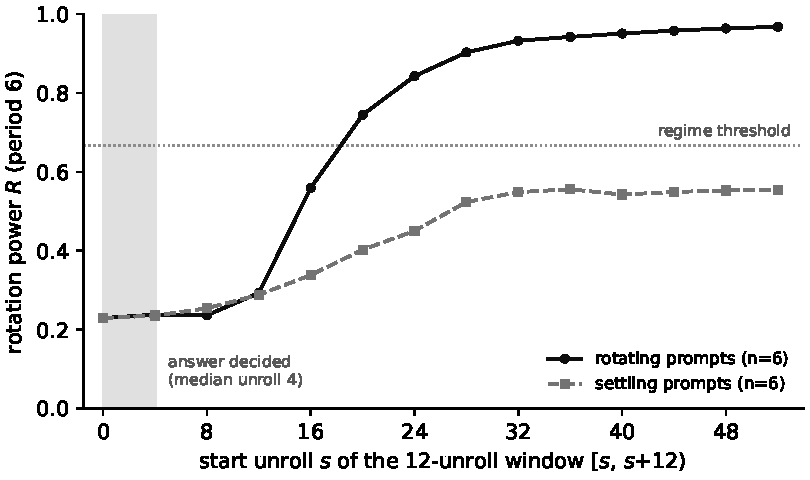
\includegraphics[width=0.68\linewidth]{pic/onset.pdf}
\caption{Rotation power in a sliding 12-unroll window, median over six rotating and six settling
prompts. The axis is the window \emph{start}: each point summarises unrolls $[s,\,s{+}12)$, twelve
being the shortest window on which a period-6 orbit is defined. The families are indistinguishable
until the window beginning at unroll~16, by which point the answer has long been settled (shaded;
median unroll~4). Higher $R$ means more power at period~6.}
\end{figure}

\subsection*{Relation to E1--E5}

The two sets of experiments use the same model, revision and hook, and they agree once the prompt
sets are taken into account.

\textbf{Why E1--E5 saw only settling.} Every prompt in E1--E5 is written in one instruction style
(``Question: \ldots{} Answer:'', ``Start at 0. Add 1. Subtract 1.\ \ldots''). E6 shows the regime is
selected by instruction wording at fixed task, fixed answer and fixed token count. So ``all 40
trajectories settle'' is what E6 predicts for that wording, and E1--E5 become a large independent
replication \emph{within the settling class} --- four task families, lengths 2--48, multiple seeds
--- rather than evidence that the model does not rotate. The results are complementary; neither is
weakened by the other.

\textbf{Two rotation measures, two scopes.} Winding is a 2D-PCA quantity, $R$ a full-space spectral
one. E1's winding null and E6's positive result are measured on different prompt sets with
different instruments and do not conflict. What the pairing shows is that a projection is fitted to
the data it judges and confounds damping with rotation, so a winding null is a weak basis for a
\emph{negative} --- a point E1--E5's own limitations already concede (``2D-PCA winding,
sign-arbitrary''). Where a negative is asserted, $R$ is the instrument that can carry it, having a
threshold validated against held-out data.

\textbf{H3.} E3's length-matched control and the position taken here are compatible and sharper
together. E3 shows effective computation grows with state retention and not with prompt length
($\rho = +0.558$ track against $-0.576$ local, both $p < 1e{-}8$). Independently, the running count
\emph{is} linearly decodable from the latents, and an untrained model carries the lagged count at
cross-validated $R^2 = 0.7498$ against the trained model's $0.7175$. Joint reading: the model
spends more compute on state-retention tasks \emph{and} the state survives contraction. What fails
is H3's strong form --- ``contraction implies the model cannot maintain a running count'' --- not
E3, which is untouched. Relatedly $\rho$ should not be quoted as a single model constant: it is
family-level, spanning $0.8239$ to $0.9181$, with between-family spread about four times the
within-family spread.

\subsection*{Limitations --- add to the existing list}

\begin{itemize}\itemsep1pt
  \item These accuracy figures and the published one compared against share an uncorrected
        surface-form bias inherent to likelihood scoring; the comparison survives it, the absolute
        values of both are questionable in the same direction.
  \item E9 says \emph{when} the properties become measurable, not \emph{whether} one influences
        the other; an intervention inside the decision window could still find an effect.
  \item A direct behavioural test of H3, injecting a donor state at $h_0$, failed three times for
        harness-internal reasons and is not reported; the authors' reported path independence over
        $h_0$ partly predicts a null there.
  \item Steering $e$ with a difference-of-means vector moved neither behaviour nor geometry
        ($|\Delta R| \le 0.0065$, zero crossings in 132 conditions, identity gate exact). The dose
        was adequate, so we read it as the wrong \emph{injection site} --- onset is 33 positions
        upstream --- not as orthogonality of directions.
\end{itemize}

\subsection*{Contribution --- add a column to the matrix}

\textbf{Arsenii Varaksin.} Rotation-power statistic and its validation; regime experiments E6
and E7; the format-versus-capability decomposition E8; the window split E9; the steering
experiment; and the instrument-null and retraction record.

\clearpage
\section*{PART 2: INTEGRATION NOTES --- NOT FOR THE PAPER}
\label{sec:notes}

\subsection*{The page budget, measured}

Stripping markup and counting body prose only, against the Zapiski text block at 330 words/page
(calibrated on a known 10-page build of the same class):

\begin{table}[h]
\centering
\small
\begin{tabular}{lcc}
\toprule
 & Words & Pages (prose only) \\
\midrule
E1--E5 body                & 1546 & $\approx 4.7$ \\
This packet, Part 1        & 1433 & $\approx 4.3$ \\
\midrule
Together                   & 2979 & $\approx 9.0$ \\
\bottomrule
\end{tabular}
\end{table}

\noindent Nine pages of prose, before the abstract and title block ($\approx 0.7$), the eight
tables in E1--E5 and the two here (0.2--0.3 each, so 2.0--2.5), the figure ($\approx 0.35$) and the
bibliography ($\approx 0.7$). Realistically the merged body lands near \textbf{12--13 pages against
a limit of 10}, so roughly 700--900 words have to come out of one side or the other. I am not in a
position to judge which of E1--E5 is expendable, so here is mine costed and ranked instead --- cut
from the bottom up.

\begin{table}[h]
\centering
\small
\begin{tabular}{lccp{6.4cm}}
\toprule
Block & W & Pp & Priority \\
\midrule
Relation to E1--E5   & 336 & 1.0 & \textbf{Essential.} Without it the merged paper contradicts itself in three places. \\
E8 (format)          & 249 & 0.8 & \textbf{Essential.} Bears directly on the 0\% counting claim (note 2). \\
E6 (regime)          & 173 & 0.5 & \textbf{Essential.} The headline result. \\
E9 (timing)          & 288 & 0.9 & Important. The hinge. Text must stay if the claim is made at all; the figure can go ($-0.35$ pp). \\
Methods insert       & 123 & 0.4 & Important. This is the winding/$R$ interface; without it E6 and E1 look like a contradiction. \\
Limitations          & 143 & 0.4 & Keep the first two bullets if pressed. \\
E7 (position)        &  85 & 0.3 & \textbf{Cut first.} A validity check, not a result. \\
Contribution         &  36 & 0.1 & Required by the venue. \\
\bottomrule
\end{tabular}
\end{table}

\noindent Dropping E7, two limitations bullets and the figure takes this to $\approx 3.3$ pages
without losing a claim. Below that, claims start going, and I would rather you tell me which than
guess. The full-length treatment of all of it is in the repository
(\texttt{docs/submission/build/main.pdf}, 10-page body), so nothing is lost from the record by
cutting here.

\subsection*{Four edits the merge needs on the E1--E5 side}

The first two are self-contradictions a reader would find inside a single document; the third is a
load-bearing evidence gap; the fourth is a scope question.

\paragraph{1. ``H2 is refuted'' has to become narrower --- highest priority.}
E1 and the conclusion read ``naive H2 is refuted'' and ``no winding-depth signal detected (naive H2
refuted)''. H2 as the adaptive-computation literature means it is \emph{per-position} depth
allocation, and Huginn has no halting head: \texttt{num\_steps} unrolls the whole sequence
together, every position receives exactly $r$, and there is nothing to allocate. The hypothesis is
not expressible on this architecture, so no null can refute it. What E1 genuinely refutes is the
\emph{winding operationalisation} --- that winding number grows with required reasoning steps.
Suggested wording: \emph{``the winding operationalisation of H2 is refuted on this prompt set; H2
in the ACT/Universal-Transformer/PonderNet sense is not expressible on an architecture without a
halting mechanism, so no experiment here bears on it.''}

\paragraph{2. ``The model fails synthetic counting (0\% at len $\ge$ 8)'' needs its scoring rule
stated.} This is the claim E8 most directly threatens, and it is load-bearing for Discussion
point~2 (``counting failure is theoretically predicted''). On our census families exact-match
scoring read $0.000$ where the answer was present in the generated text in $78.1\%$ of cases; a
$0\%$ reading on this model is exactly what a formatting confound produces. If the counting
accuracy came from exact match or a first-token/fixed-parser rule, the banked generations should be
re-scored by containment before the capability claim stands. It may well survive --- parity and
state tracking are predicted to fail on theoretical grounds --- but the number needs the format
control, or the claim should read ``fails under exact-match scoring'' with the rule named.

\paragraph{3. The Pappone refutation should be split by which arm supports it.}
Two different experiments currently sit under one heading: a \emph{synthetic} arm (depths 2--5,
orthogonality $\approx -0.5$, exits fixed at 50\%) run on a purpose-built 128-dimensional recurrent
autoencoder trained for 50 epochs, and a \emph{FineWeb} arm on real text ($\cos \approx -0.687$).
Only the second can speak to Pappone et al., whose claim concerns recurrent-depth transformers. The
toy model also \emph{initialises} its rotation layer orthogonally
(\texttt{nn.init.orthogonal\_}), so orthogonal structure there is partly imposed by construction
rather than discovered --- worth one clause, because a reviewer who opens the notebook will see it.
Suggested split: keep ``step normalisation is required for a clean orthogonality measurement'' as
the methodological finding, which both arms support and which is the genuinely useful result;
restrict ``refutes the universality of Pappone et al.'' to the FineWeb arm.

\emph{A correction I owe on this:} I earlier flagged the README's $-0.687$ as inconsistent with the
$-0.494$ in \texttt{two\_scale\_real.csv}. That was wrong. They are two different experiments ---
FineWeb real text and synthetic depths 2--5 respectively --- and both tables in the paper are
internally consistent. The filename misled me.

\paragraph{4. Duplicate material to delete on merge.}
Both drafts carry a ``Model and Protocol'' paragraph naming the same revision
(\texttt{bb6621b6...}) and the same \texttt{core\_block[-1]} hook; keep one. Four bibliography
entries are shared and will duplicate: Geiping, Bai (DEQ), Grazzi, Pappone. The E1--E5 draft cites
Merrill (2404.08819) for ``illusion of state'' and Grazzi (2411.12537) for parity, which is
correct --- do not let a merge collapse them, since an earlier draft of ours cited 2404.08819 for
the parity claim and that was a misattribution we had to fix.

\paragraph{Not a conflict, worth one sentence.} The limitation ``Geiping regime not reproduced ---
we did not use their system prompt or $r=128$'' now has a partial answer: the system turn is not
the missing ingredient. The identical instruction text in the system turn rather than the user turn
buys one item in twenty-four, paired, $p = 1.0$.

\subsection*{On the compliance items, since the merge changes who owns them}

The venue requires a Contribution section with one entry per team member (stated twice in the
instructions), all authors registered on OpenReview, and mentors listed. The E1--E5 contribution
matrix currently has columns only for Shiianov and Sverdlov; it needs a third. The acknowledgments
there thank S.\ Barannikov and N.\ Kurdyukov, while our draft lists Barannikov as mentor --- worth
agreeing which is correct before upload, as it is a stated requirement rather than a matter of
taste.

\end{document}
